% !TeX spellcheck = fr-FR

\documentclass[10pt,a4paper,notitlepage ]{article}

\usepackage{pfmath}
\usepackage{listings}


\title{Systèmes numériques - \textsc{Ernest'O'Clock}}
\date{Premier semestre 2020}
\author{Paul \textsc{Fournier}, Juliette \textsc{Schabanel}, Samuel \textsc{Vivien}}

\lstset{
	backgroundcolor=\color{yellow!5!white},
	keywordstyle=\color{violet!80!black},
	numbers=left,
	frame=single,
	numberstyle=\tiny\color{violet!80!black},
	escapeinside={\%*}{*)},
	stringstyle=\color{black!20!yellow},
	morecomment=[l][\color{green}]{\$}
}

\begin{document}
	\selectlanguage{french}
	\pagenumbering{gobble}
	\maketitle
	\pagebreak
	\pagenumbering{roman}
	\tableofcontents
	\pagebreak
	\pagenumbering{arabic}
	
	\section{Utilisation de l'horloge}

		Il a y 4 commandes dans le makefile qui sont utile pour l'utilisation de l'horloge :

		\begin{itemize}
			\item \texttt{make} qui va simplement build l'exécutable de l'horloge.
			\item \texttt{make run} qui va build l'exécutable si il ne l'est pas déjà, puis la lancer.
			\item \texttt{make speed} qui fait la même chose que la commande précédente pas avec le mode hyper-vitesse.
			\item \texttt{make clean} qui nettoie tout (mais nettoie moins que \texttt{rm -rf $\backslash$ }).
		\end{itemize}

	\section{Compilation $\tt{.net} \rightarrow \tt{.c}$}
	
	\subsection{Motivations}
	
	De prime abord, nous avions implémenté un simulateur de netlist, codé en \texttt{OCaml}, mais nous avons décidé de changer et de produire un code \texttt{C} ayant le même comportement que la netlist d'entrée, et ce pour deux raisons.
	\begin{enumerate}
		\item Les performances de \texttt{C}, en particulier grâce à l'optimisation apportée par \texttt{gcc}.
		\item Le côté bas niveau permet de gérer plus facilement les entrées/sorties de l'ordinateur/simulateur/émulateur.
		\item Avons-nous mentionné \texttt{gcc} ?
	\end{enumerate}
	
	\subsection{Implémentation}
	
	Le compilateur est implémenté en \texttt{OCaml}, parce que la plupart du code en amont l'était déjà, ce qui permet d'éviter des interfaces inutiles et lourdes.
	
	L'idée est assez simple finalement, en \texttt{C}, on alloue un énorme tableau, dont chaque case est un fil, un tableau par RAM, et un tableau par ROM. Les opérations sur les netlist se transforment alors par un isomorphisme presque immédiat en opération sur les tableaux.
	
	\subsubsection{Les fils}
	
	Nous donnons ici rapidement les idées derrière la traduction des opérations sur des fils simples.
	
	\begin{center}
		
	\begin{tabular}{|c|c|}
		\hline
		Opérations sur les fils & Opérations sur les tableaux \\
		\hline
		Constante (\texttt{true} ou \texttt{false})& Constante ($0$ ou $1$)  \\
		\hline
		\texttt{not a}& \texttt{!a}  (nb: plus rapide qu'un \texttt{xor})\\
		\hline
		\texttt{and} & \texttt{\&}  \\
		\hline
		\texttt{or}& \texttt{|} \\
		\hline
		\texttt{xor}& \texttt{\^} \\
		\hline
		\texttt{a nand b }& \texttt{!(a \& b)} \\
		\hline
		\texttt{mux s b a}& \texttt{s?a:b} \\
		\hline
		\texttt{reg}&Assignation\\
		\hline
	\end{tabular}
	
	\end{center}

	\subsubsection{Les RAM}
	
	Chaque RAM est un tableau. La lecture est simplement la lecture des cases du tableau, et l'écriture, sans grande surprise, l'écriture dans les cases du tableau.
	
	Les opérations sont effectuées bit à bit, il pourrait donc y avoir quelques optimisations à effectuer de ce côté là (en écrivant par blocs de puissances de deux par exemple).
	
	Pour des questions d'utilisation mémoire du simulateur, et comme nous n'avons pas implémenté de tables de hachage en \texttt{C}, la taille de la RAM est bornée, par une quantité prédéfinie, mais modifiable par un argument optionnel au moment de la compilation.
	
	Si une adresse non valide est spécifiée, le CPU lève un \texttt{SEGFAULT}.
	
	\subsubsection{Les ROM}
	
	Étant immuables, les ROM sont définies en dur dans le code \texttt{C} généré par le compilateur (par exemple, aux alentours des lignes  $\sim$ 150 du code produit pour notre CPU, on peut trouver la ROM comprenant le code à exécuter, telle les disquettes des anciens).
	
	On peut donc y lire, comme dans une RAM, et si une adresse invalide est spécifiée (ex: fin du programme), l'exécution s'arrête proprement.
	
	
	\section{Microprocesseur}

		\subsection{Le design}

		Le microprocesseur a été construit de façon très simple, ayant dans l'esprit que l'on essayait de faire quelque chose de simple avec peu d'instructions et beaucoup de registres à la \texttt{RISC-V}. Nous avions un code \texttt{minijazz} fonctionnel pour la multiplication, cependant nous avons décidé de ne pas l'ajouter à notre microprocesseur pour gagner en efficacité.

		Le microprocesseur a donc été construit autour d'un $n$-adder. Qui nous permettait à l'aide d'une série de multiplexeurs de faire les opérations d'addition, soustraction, incrémentation, décrémentation. Nous avons rajouté à côté de cela les opérations booléennes et les décalages à droite et à gauche.

		Nous avons aussi pris la décision d'opter pour 32 registres de 32 bits, ainsi que 4 flags (carry, overflow, isNeg et notZero).

		De plus afin de nous simplifier la vie nous avons décider de séparer la RAM permettant de stocker des données, de la ROM qui avait pour but de contenir le code.

		Nous avons eu alors un problème : comment charger des valeurs de 32 bits dans une instruction de 32 bits. Nous avons donc décidé de créer ce que nous avons appelé le Demi-registre. Un registre 16 bits qui contient la moitié de l'instruction du cycle précédent. Permettant ainsi de charger en deux cycle une grande valeur. Pour les petites valeurs, il nous suffisait d'indiquer de l'on devait compléter notre valeur de 16bits par des zéros.

		\subsection{Le code machine}

		Une instruction machine se décompose en 5 parties : 
		\begin{enumerate}
			\item L'opération codé sur les 7 premiers bits. Il s'agit du parcours dans l'arbre de multiplexeur permettant de nous ramener à la bonne valeur. Nous n'utilisons pas tous les bits pour nos instructions ce qui nous permettrais d'en rajouter plus si besoin.

			\item Sur le $8$\ieme bit se situe l'ordre d'écrire ou non le résultat du calcul. Permettant ainsi de différencier les \textbf{and} et \textbf{sub} des instructions \textbf{test} et \textbf{cmp}.

			\item La valeur d'entrée sur $16$ bits. Il peut s'agir d'une valeur numérique, ou du numéro d'un registre. Cette valeur est sauvegardé dans le demi-registre pour le cycle suivant.

			\item Le type de l'entrée est ensuite implémenté sur $2$ bits pour indiquer si il s'agit d'un registre, de la valeur pointée par un registre ou simplement d'une valeur numérique (étendu avec des zéros ou la valeur dans le demi-registre).

			\item Ensuite se situe la valeur de sortie sur 5 bits, car il s'agit forcément de l'indice d'un registre.

			\item Et pour finir sur le $32$\ieme bit, une indication sur si il s'agissait de la valeur du registre ou l'emplacement en mémoire pointé par le registre qui nous intéresse
		\end{enumerate}


\section{Langage assembleur}
\subsection{Le langage}
	\par{Nous avons créé notre langage assembleur en nous inspirant fortement du langage \texttt{x86-64}. Il comporte un jeu d'instructions plus restreint qui sont les suivantes :
	\begin{itemize}
		\item \texttt{add} $x \text{ } y \rightarrow x := x + y$
		\item \texttt{sub} $x \text{ } y \rightarrow x := x - y$
		\item \texttt{neg} $x \rightarrow x := - x $
		\item \texttt{and} $x \text{ } y \rightarrow x := x \&\& y$
		\item \texttt{or} $x \text{ } y \rightarrow x := x || y$
		\item \texttt{xor} $x \text{ } y \rightarrow x := x ^ y$
		\item \texttt{not} $x \rightarrow x := \neg x$
		\item \texttt{lsl / lsr} $x \text{ } n \rightarrow $ logical shift de $n$
		\item \texttt{asr} $x \text{ } n \rightarrow $ arithmetical shift de $n$
		\item \texttt{incr} $x \rightarrow x := x + 1$
		\item \texttt{decr} $x \rightarrow x := x - 1$
		\item \texttt{mov[flag]} $x \text{ } y \rightarrow x := y$ conditionné par le drapeau
		\item \texttt{jmp / j[flag]} $label \rightarrow $ saut (conditionnel) vers le label
		\item \texttt{cmp} $x \text{ } y \rightarrow $ donne aux drapeaux les valeurs pour $x - y$
		\item \texttt{test} $x \text{ } y \rightarrow $ donne aux drapeaux les valeurs pour $x \&\& y$
	\end{itemize}
	Les registres sont des registres 32 bits et sont au nombre de 32. Ils sont nommés de \texttt{r00} à \texttt{r31}, les trois derniers ayant pour alias respectivement \texttt{rsp, rbp} et \texttt{cpp}\\
	Les différents drapeaux autorisés sont :
	\begin{itemize}
		\item \texttt{e} : nullité du résultat [ZF]
		\item \texttt{ne} : non nullité [$\neg$ ZF]
		\item \texttt{s} : résultat négatif [SF]
		\item \texttt{ns} : résultat positif [$\neg$ SF]
		\item \texttt{g} : > [$\neg$(SF xor OF) \& $\neg$ ZF] 
		\item \texttt{ge} : $\geqslant$ [$\neg$(SF xor OF)]
		\item \texttt{l} : < [SF xor OF]
		\item \texttt{le} : $\leqslant$ [(SF xor OF)|ZF]
		\item \texttt{a} : > non signé [$\neg$ CF \& $\neg$ ZF]
		\item \texttt{ae} : $\geqslant$ non signé [$\neg$ CF]
		\item \texttt{b} : < non signé[CF]
		\item \texttt{be} : $\leqslant$ non signé [CF$\vert$ZF]
	\end{itemize}}
	\par{La syntaxe  est calquée sur celle de x86-64 :
	\begin{itemize}
		\item[$\bullet$] $\%<nom \text{ } du \text{ } registre>$ pour désigner la valeur contenue dans un registre.
		\item[$\bullet$] $(\%<nom \text{ } du \text{ } registre>)$ pour désigner la valeur contenue en mémoire à l'adresse contenue dans le registre, un seul de ces accès mémoire est autorisé par instruction
		\item[$\bullet$] $\$<entier>$ pour les constantes.
		\item[$\bullet$] $<label>:$ pour poser un label et $"<label>"$ pour y sauter, les caractère autorisés pour les noms de labels sont les lettres majuscule et minuscules de l'alphabet latin, '\_' et les chiffres hors première caractère (i.e. \texttt{(['a'-'z' 'A'-'Z'] $\vert$ '\_') (['a'-'z' 'A'-'Z'] $\vert$ '\_' $\vert$ ['0'-'9'])*}).
		\item[$\bullet$] $\#$ pour désigner le début d'un commentaire, tout le texte suivant un $\#$ sera ignoré jusqu'au premier retour à la ligne.
	\end{itemize}
	La grammaire est décrite simplement par les règles suivantes :
	$$\begin{array}{rcl}
		<mem> & = & \%<register> | (\%<register>) \\
		<param> & = &  \%<register> | (\%<register>) | \$<entier>\\
		<instr> & = & <operateur> <mem> <param>? \\
		& | & mov <flag>? <mem> <param> \\
		& | & jmp <flag>? "<label>" \\
		& | & <label> : \\ 
	\end{array}$$}
		
\subsection{Compilation}
	\par{Nous avons codé un assembleur qui assemble notre langage assembleur vers notre langage machine en utilisant OCaml, et en particulier \texttt{ocamllex} pour le lexer et \texttt{menhir} pour le parser. Notre compilateur vérifie que la limite d'une accès mémoire par instruction n'est pas dépassée et la présence d'un registre en argument quand celle-ci est requise.}


	\section{Interface homme machine}
	
	Nous allons ici détailler la façon dont nous avons implémenté l'interface entre le microprocesseur, qui, après calcul, donne une représentation du temps sous format sept segments.
	
	\begin{figure}[h]
		\centering
		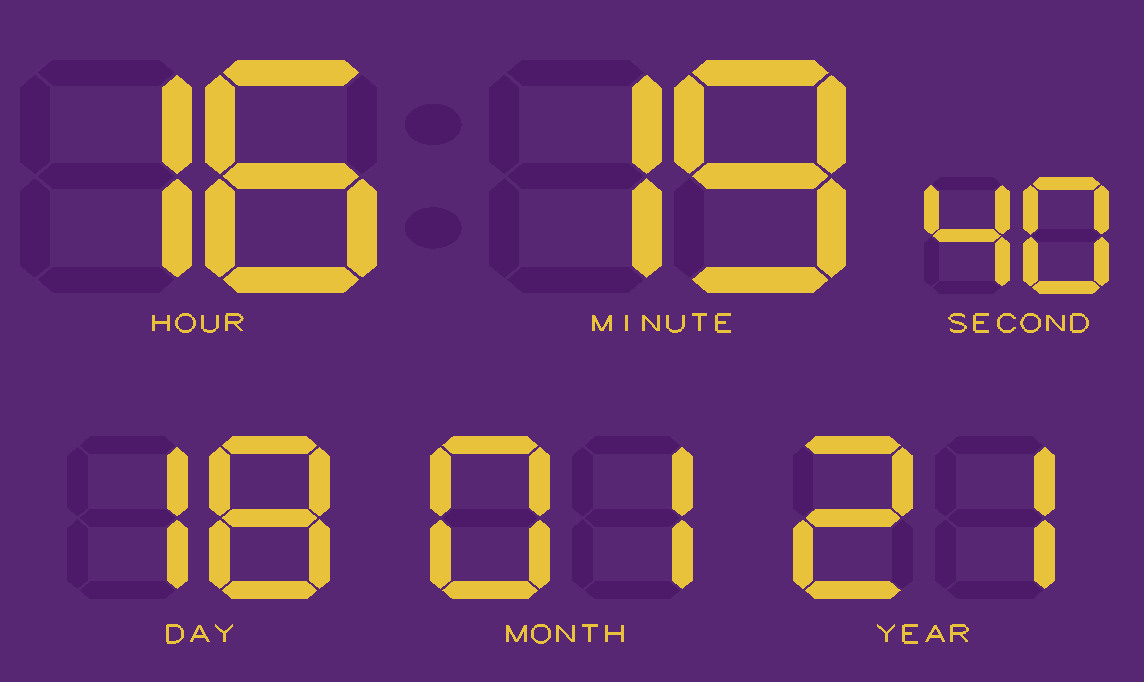
\includegraphics[width=0.7\linewidth]{2021-01-18_16-19}
		\caption{Capture d'écran de la sortie de l'horloge}
		\label{fig:2021-01-1816-19}
	\end{figure}
	
	Commençons par expliquer comment nous avons réalisé l'affichage en lui-même.
	
	\subsection{Programmation graphique de l'horloge}
	
	Ils a donc d'abord fallu décider d'une façon d'encoder en mémoire les segments. Pour cela, chaque chiffre est représenté par un mot de $7$ bits (donc en pratique par un octet). La figure ci-dessous détaille quel bit correspond à quel segment (avec le mot indicé comme $b_0b_1b_2b_3b_4b_5b_6b_7$).
	
	\begin{figure}[h]
		\centering
		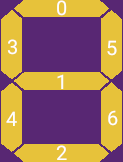
\includegraphics[width=0.3\linewidth]{segments}
		\caption{Encodage des segments}
		\label{fig:segments}
	\end{figure}
	
	L'interface s'est effectuée directement par une lecture dans la RAM. Une section "MMIO" a été définie et réservée pour cela. C'est concrètement du repiquage de fil de la mémoire vers un afficheur à cristaux liquide, mais virtualisé dans le code \texttt{C}.
	
	Maintenant qu'on a récupéré le statut "on/off" de chaque segment, il est temps de l'afficher !
	
	Nous avons choisi d'utiliser \texttt{OpenGL} comme libraire graphique. Ce choix a été motivé principalement parce que nous avions déjà (un peu) d'expérience avec cette librairie et que cela permettait de gagner en efficacité pendant la production. Par ailleurs, c'est une libraire répandue et connue, ce qui nous a évité de chercher pendant des heures comment faire pour afficher quelques bâtons sur un écran. Cependant, bien que nous avons voulu, en gardant le code assez simple, optimiser autant que faire se peut la vitesse d'affichage, $\tt{OpenGL}$ restant une libraire de rendu 3D à l'origine, il est évident que les opérations matricielles à répétition qu'engendrent le positionnement des différents éléments sur l'écran sont probablement sous-optimaux par rapport à une librairie spécialisée dans l'affichage rapide de forme géométrique simples en deux dimensions.
	
	Comme il y a 3 formes à afficher (segment horizontal, segment vertical et point), nous avons décidé d'utiliser les "display list" pour stocker en mémoire les formes et les répliquer plus rapidement par la suite. Nous n'avons pas relevé expérimentalement de différence, mais c'est considéré comme une bonne pratique par l'ouvrage qui nous a servi de référence (OpenGL programming guide - The official guide to learning OpenGL). Ensuite, c'est juste du placement minutieux de chaque segment. Les détails précis de la position ne seront pas explicités ici (long, moche, pénible, et inutile au propos), ils sont cela dit consultable depuis le code source, pour nos lecteurs masochistes. En fait, en interne, à chaque placement, \texttt{OpenGL} fait un produit matriciel $4\times 4$, ce qui pourrait en pratique être simplifié en utilisant autre chose qu'un moteur 3D.
	
	Finalement, à chaque frame, \texttt{OpenGL} affiche $7\times 12$ segments, et deux points, de la couleur adaptée (allumé, éteint, selon le seul code couleur qui vaille la peine d'être implémenté) en plus du texte.
	
	\subsection{Entrées du microprocesseur}
	
	Afin d'interagir avec le monde, le microprocesseur doit aussi prendre des entrées. Pour le projet d'horloge, il s'agit d'une information d'initialisation - l'heure initiale -, et d' une information en temps réel - la parité de la seconde actuelle.
	
	L'heure initiale est donnée sous la forme d'un entier 32 bits, encodé classiquement, contenant le nombre de secondes depuis le premier Janvier 1970 (UNIX epoch). Le microprocesseur fait toutes les conversions nécessaires en interne.
	
	Ensuite, le bit de parité de la seconde en cours (qui sert aussi pour faire clignoter les deux points séparant les minutes des secondes), est calé entre deux paquets de sept bits dans le MMIO, bien au chaud.
	
	\subsection{Optimisations pour le mode \textit{hyper-vitesse}}
	
	Lors des premiers tests, nous avons remarqué que l'affichage était le facteur limitant en termes de vitesse d'affichage, pas le CPU. C'est pour cela que nous avons voulu passer un peu de temps à réduire le temps passé à afficher des choses à l'écran.
	
	Pour cela, nous avons ajouté un bit dans l'interface MMIO (toujours calé entre deux blocs de sept), qui est envoyé par le CPU lorsque les calculs sont terminés pour une unité de temps, qui dit concrètement au front-end "fin de la pause, il faut mettre à jour l'affichage de l'heure". Une fois que l'affichage est réalisé, ce bit est remis à zéro.
	
	\subsection{Lecture des inputs de l'utilisateur}
	
	Les entrées clavier de l'utilisateur sont lues lors de l'exécution de l'horloge et que le processus est en avant-plan. Actuellement, tout ce qui est vérifié est l'appui des touches \texttt{Q} et \texttt{MAJ} en simultané, ce qui ferme le programme.
	
	\subsection{Autres idées non implémentées}
	
	Nous avions d'autres projets pour cette partie d'interface. En particulier, nous voulions enrichir l'entrée utilisateur. Des tests en local (\texttt{hexdump}, entre autres) nous ont permis de conclure qu'il était, effectivement, possible de faire ce qui est ni plus ni moins qu'un keylogger en lisant directement dans \texttt{/dev/input}. Nous avons testé, et il était possible de récupérer les informations de :
	\begin{itemize}
		\item Trackpad
		\item Clics
		\item Clavier
		\item Manette de \textsc{Nintendo} Switch\texttrademark\ type Game Cube (connectique USB)
	\end{itemize}
	
	Le code utilisé pour tester peut être trouvé en annexe.
	Il aurait alors été possible, avec un peu de traitement, certes, de donner des informations plus complexes au CPU. 
	
	Nous aurions aussi voulu modifier le système d'affichage pour pouvoir avoir du contrôle directement sur les pixels mêmes de l'écran. Là aussi, nous aurions voulu aller fouiner du côté du noyau Linux, mais c'est une magie encore trop ésotérique pour nous. Nous aurions aussi pu chercher une librairie qui gère de l'affichage 2D, mais le temps nous a manqué.
	
	L'objectif final aurait été de pouvoir avoir une machine qui a des performances comparables à celles des premières consoles de jeu, et montrer ses performances en implémentant un petit jeu type Snake ou Pong.
	
	De manière orthogonale, nous aurions aussi aimé, quitte à utiliser \texttt{OpenGL}, pouvoir faire profiter l'utilisateur de l'horloge d'un environnement 3D composé essentiellement d'une table de chevet sur laquelle repose un radio-réveil (notre horloge).
	

	\section{Horloge}

		\subsection{Initialisation}

			Une partie relativement technique de l'implémentation de l'horloge résidait dans son initialisation. À partir du nombre de secondes depuis le début de l'univers (a.k.a. le premier janvier 1970), il fallait tout décomposer pour avoir l'heure en :
			\begin{itemize}
				\item unité des secondes,
				\item dizaine des secondes,
				\item unité des minutes,
				\item dizaines des minutes,
				\item et cetera, jusqu'au siècle.
			\end{itemize}

			Pour cela le plus simple est de faire une division euclidienne. Une instruction que nous n'avions pas implémenté dans le microprocesseur. Il a donc fallut l'implémenter en assembleur à l'aide de comparaison et décalages logiques.

			Si vous vous souvenez de comment vous avez appris à faire des division euclidienne en primaire. Alors vous avez juste à convertir le même algorithme mais qui fonctionne en base 2 pour obtenir notre division euclidienne.

			Voici donc le code assembleur de notre division euclidienne qui fait la division de la valeur dans \texttt{\%r28} par 86400. Avec le reste dans \texttt{\%r28} et le quotient \texttt{\%r27}

\begin{lstlisting}[language={[x86masm]Assembler},morekeywords={lsr}]
	mov %r26 $86400
	mov %r25 %r26
	jmp "ew1"
%*\texttt{bw1:}*)
	lsl %r25 $1
ew1:
	cmp %r28 %r25
	jb "bw1"
	mov %r27 $0
bw2:
	lsl %r27 $1
	cmp %r28 %r25
	ja "ew2"
	add %r27 $1
	sub %r28 %r25
ew2:
	lsr %r25 $1
	cmp %r25 %r26
	jge "bw2"

\end{lstlisting}

\subsection{Incrémentation}
	\par{Le tic d'horloge est donné sur le bit d'indice $31$ de la RAM sous la forme d'un changement de valeur à chaque seconde. Notre programme récupère cette valeur à chaque boucle et la compare à la dernière valeur lue, pour savoir si il doit incrémenter le temps. \\
	Pour faciliter le traitement, chaque chiffre est stocké dans un registre différent. On utilise en plus un registre stockant le numéro du mois en entier et de même pour l'année, ainsi qu'un dernier indiquant si l'année est bissextile ou non.\\ 
	On commence par incrémenter le chiffre des unités des secondes, le compare à 10, si il est strictement inférieur on saute directement à l'affichage et sinon on incrémente les dizaines, et ainsi de suite jusqu'à la fin de la propagation. Pour savoir si l'on change de mois on non après avoir incrémenté le jour, nous avons cherché à déterminer le nombre de jours du mois en un minimum de test, ce qui nous à conduit à l'arbre de test suivant où pour chaque nœud interne, le fils gauche correspond à un \texttt{false} et le droit à un \texttt{true} :
	$$
	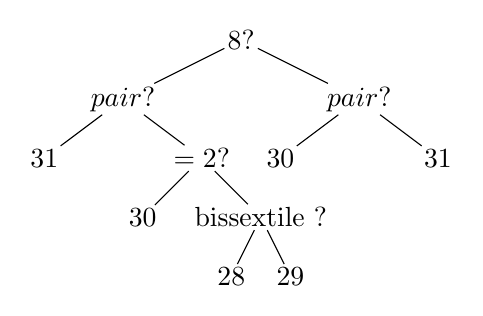
\begin{tikzpicture}[baseline = -20pt, level distance = 0.75cm, level 1/.style={sibling distance=3cm},
                   level 2/.style={sibling distance=2cm},
                   level 3/.style={sibling distance=1.5cm},
                   level 4/.style={sibling distance=0.75cm}]
	\begin{scope}[every node/.style={fill=white, inner sep=1pt}]
	\node {$\geqslant 8\text{ ?}$}
	 child {node {$\text{pair ?}$}
	        child {node{$31$}}
	        child {node{$= 2\text{ ?}$}
	        		child {node{$30$}}
			child {node{\text{bissextile ?}}
				child {node{$28$}}
				child {node{$29$}}
				}
			}
	       }
	 child {node {$\text{pair ?}$}
	 	child {node{$30$}}
		child {node{$31$}}
		}
	      ;
	\end{scope}
	\end{tikzpicture}
	$$}


\subsection{Output}
	\par{Pour terminer la boucle, on convertit chaque chiffre en une séquence de 7 bits indiquant quels segments doivent être allumés. Pour économiser quelques cycles, nous avons cherché à minimiser le nombre de tests, ce qui nous a conduit à l'arbre de test suivant, $s_i$ représentant le $i$-ème bit : \\
	$$
	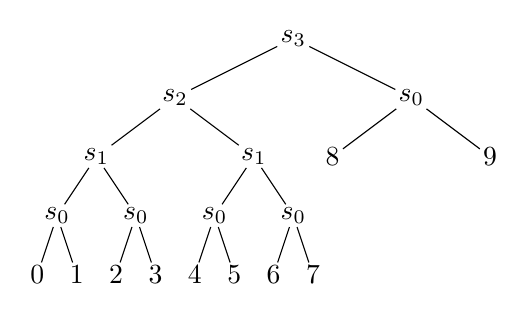
\begin{tikzpicture}[baseline = -20pt, level distance = 0.75cm, level 1/.style={sibling distance=3cm},
                   level 2/.style={sibling distance=2cm},
                   level 3/.style={sibling distance=1cm},
                   level 4/.style={sibling distance=0.5cm}]
	\begin{scope}[every node/.style={fill=white, inner sep=1pt}]
	\node {$s_3$}
	 child {node {$s_2$}
	        child {node{$s_1$}
	        		child {node{$s_0$}
				child {node{$0$}}
				child {node{$1$}}
				}
			child {node{$s_0$}
				child {node{$2$}}
				child {node{$3$}}
				}
			}
	        child {node{$s_1$}
	        		child {node{$s_0$}
				child {node{$4$}}
				child {node{$5$}}
				}
			child {node{$s_0$}
				child {node{$6$}}
				child {node{$7$}}
				}
			}
	       }
	 child {node {$s_0$}
	 	child {node{$8$}}
		child {node{$9$}}
		}
	      ;
	\end{scope}
	\end{tikzpicture}
	$$
	Le résultat est ensuite placé sur la RAM. Pour optimiser l'espace, les chiffres sont regroupés par quatre et le résultat est écrit sur les trois premières cases de la RAM. On termine en donnant au bit 30 la valeur 1 pour signaler à l'affichage qu'il faut effectuer un rafraîchissement.}

	\begin{figure}
	\begin{lstlisting}[language=C, frame=single, caption={Keylogger test}]
#include <stdlib.h>
#include <stdio.h>
#include <string.h>
#include <errno.h>
#include <linux/input.h>
#include <sys/types.h>
#include <sys/stat.h>
#include <fcntl.h>
#include <libevdev/libevdev.h>
#include <libevdev/libevdev-uinput.h>

int main(){
	
	struct libevdev *dev = NULL;
	int fd;
	int rc = 1;
	
	// keyboard : /dev/input/event3
	//fd : file descriptor
	fd = open("/dev/input/event3", O_RDONLY|O_NONBLOCK);
	// rc : return code
	// modifies *dev such that it is hooked to the /dev/input file
	rc = libevdev_new_from_fd(fd, &dev);
	if (rc < 0) {
		//error happenned
		fprintf(stderr, "Failed to init libevdev (%s)\n", strerror(-rc));
		exit(1);
	}
	printf("Input device name: \"%s\"\n", libevdev_get_name(dev));
	printf("Input device ID: bus %#x vendor %#x product %#x\n",
	libevdev_get_id_bustype(dev),
	libevdev_get_id_vendor(dev),
	libevdev_get_id_product(dev));
	
	do {
		struct input_event ev;
		rc = libevdev_next_event(dev, LIBEVDEV_READ_FLAG_NORMAL, &ev);
		if (rc == 0)
		printf("Event: %s %s %d\n",
		libevdev_event_type_get_name(ev.type),
		libevdev_event_code_get_name(ev.type, ev.code),
		ev.value);
	} while (rc == 1 || rc == 0 || rc == -EAGAIN);
	0;
}
	\end{lstlisting}
	\end{figure}


\newpage

Codification du langage machine, les étoiles signifient que l'on peut mettre librement un 0 ou un 1 sans que cela change l'instruction.

\begin{enumerate}

\item Le code sur 7 bits

\begin{itemize}

\item ******1 si calcul
\begin{itemize}
\item *****11 -> arithmétique
\begin{itemize}
\item ****011 -> Additions
\begin{itemize}
\item 00**011 -> add
\item 01**011 -> sub
\item 10**011 -> incr
\item 11**011 -> decr
\end{itemize}

\item ****111 -> Décalages
\begin{itemize}
\item 00**111 -> lsl
\item 01**111 -> lsr
\item 11**111 -> asr
\end{itemize}
\end{itemize}

\item *****01 -> logique
\begin{itemize}
\item ****001 -> calcul booléen
\begin{itemize}
\item 00**001 -> and
\item 01**001 -> or
\item 10**001 -> nand
\item 11**001 -> xor
\end{itemize}
\end{itemize}

\begin{itemize}
\item ****101 -> not et minus
\begin{itemize}
\item ***0101 -> not
\item ***1101 -> minus
\end{itemize}
\end{itemize}
\end{itemize}
\item ******0 si mov
\begin{itemize}
\item 0000**0 -> move
\item 1000**0 -> movne
\item 0100**0 -> movs
\item 1100**0 -> movns
\item 0010**0 -> movge
\item 1010**0 -> movg
\item 0110**0 -> movle
\item 1110**0 -> movl
\item 0001**0 -> movae
\item 1001**0 -> mova
\item 0101**0 -> movbe
\item 1101**0 -> movb
\item **11**0 -> mov
\end{itemize}

\end{itemize}

\item write\_enable

1 pour écire, 0 sinon

\item Entrée sur 16 bits

si c'est un entier mettre en binaire avec les bits de poids fort à gauche.

\item Type de l'entrée (imm, reg, mem):
	\begin{itemize}
		\item 00 -> valeur binaire avec des 0 au début : 000... param2
		\item 01 -> valeur binaire avec le demi-registre au début : demiR.param2
		\item 10 -> valeur registre
		\item 11 -> valeur pointé par le registre
	\end{itemize}

Le demi-registre contient la valeur du param2 du cycle précédent.

\item Sortie sur 5 bits

Valeur en base 2 de l'indice du registre lu

\item Type de la sortie (reg, mem)

1 si dans la mémoire, 0 sinon


\end{enumerate}

\end{document}
